% !TeX document-id = {5f9589b8-498a-4233-98c1-605de3ca7afa}
% !TeX TXS-program:compile = txs:///pdflatex/[--shell-escape]


\documentclass[12pt, paper=a4, bibtotoc, toc=listof]{scrreprt}
\setcounter{tocdepth}{3}% Include \subsubsection in ToC
\setcounter{secnumdepth}{3}% Number \subsubsection
\setuptoc{toc}{numbered} % Adds ToC to ToC toDo: remove Pagenumber of ToC in ToC

\usepackage[ngerman]{babel} %Deutsch

\usepackage[utf8]{inputenc} %UTF8 Formatierung

\usepackage[T1]{fontenc}

\usepackage{helvet} %Arial
\renewcommand{\familydefault}{\sfdefault} %Arial

\usepackage{float}
\newfloat{listing}{tbhp}{lst}%[section]
\floatname{listing}{Listing}
\newcommand{\listoflistings}{\listof{listing}{Listing Verzeichnis}}

\usepackage{chngcntr}% http://ctan.org/pkg/chngcntr
\counterwithin{listing}{chapter} %counts chapters of listing




\usepackage[chapter]{minted} %Code Formatierung
\newminted{JavaScript}{frame=single,framesep=10pt}
\newminted{HTML}{frame=single,framesep=10pt}

\usepackage{caption}
\DeclareCaptionFont{black}{\scriptsize\color{black}}
\DeclareCaptionFormat{listing}{{\parbox{\linewidth-2\fboxsep}{#1#2#3}}}
\captionsetup[listing]{labelfont=black,textfont=black} %Caption of Listing
\captionsetup[figure]{labelfont=black,textfont=black} %Caption of Figure

\usepackage{graphicx} %IMG

\usepackage{csquotes}

\usepackage[onehalfspacing]{setspace} %Zeilenabstand


\usepackage[
	backend=biber,
	style=numeric
	]{biblatex}
\addbibresource{library.bib}

\usepackage{acronym}


% Neues cite-Kommando oder altes \footcite-Kommando überschreiben
\DeclareCiteCommand{\smfootcite}[\mkbibfootnote]
{\usebibmacro{prenote}}                                 
{\usebibmacro{citeindex}%
	\setunit{\addnbspace}
	\printnames{labelname}%
	\setunit{\labelnamepunct}
	\newunit
	\printfield{year}
}
{\addsemicolon\space}
{\usebibmacro{postnote}}


\title{Erstellung von adaptiven Web Components}
\author{Christoph Kleber}
\date{\today}

\begin{document}

	\maketitle
	
	\chapter*{Kurzfassung}
	\addcontentsline{toc}{chapter}{Kurzfassung}
	In dieser Arbeit geht es um Web Components.
	
	\chapter*{Abstract}
	\addcontentsline{toc}{chapter}{Abstract}
	
	This thesis is about Web Components.
	\listoflistings
	\listoffigures
	\chapter*{Abkürzungsverzeichnis}
	\addcontentsline{toc}{chapter}{Abkürzungsverzeichnis}
		\begin{acronym}
		\acro{API}{Advanced Programming Interface}
		\acro{DOM}[DOM]{Document Object Model}
		\acro{HTML}[HTML]{Hypertext Markup Language}
		\acro{URL}[URL]{Uniform Resource Locator}
		\acro{div}[div]{division}
		\acro{HTML5}[HTML5]{Hypertext Markup Language Version 5}
		\acro{CSS}[CSS]{Cascading Style Sheets}
	\end{acronym}

	\tableofcontents
	

	\chapter{Adaptivität}
		\section{Begriffsklärung}
			Das ist erster Text
			Test
	

		\section{Adaptivität bei User Interfaces}
	\chapter{Web Components}
		\section{Was sind Web Components}
		
		\section{Geschichte von Web Components}
		\section{Gegenüberstellung Webentwicklung ohne und mit Web Components}
		\section{Technik der Web Components}
			\subsection{Custom Elements}
			Das \emph{Custom Element} ist eine \emph{\ac{API}}, welches das Bilden eigener, voll funktionstüchtiger \emph{\ac{DOM}} Elemente ermöglicht.\smfootcite[ vgl. ][]{Denicola2016} Die \emph{\ac{API}} beschreibt in diesem Zusammenhang eine Schnittstelle, welche einem anderen Programm ein Tool zur Verfügung stellt, um sich an das eigene Softwaresystem anbinden zu können.\smfootcite[ vgl.][]{Behrendt2016} Somit ermöglicht eine \emph{\ac{API}} einen Austausch von Informationen zwischen verschiedenen Programmen oder Systemen.	
			Die \emph{Custom Element \ac{API}} ermöglicht den Nutzern die Auszeichnungsprache \emph{\ac{HTML}} zu erweitern.\smfootcite[ vgl.][]{Argelius2016} Es können bestehende \emph{\ac{HTML}} Elemente erweitert, oder neue hinzugefügt werden. Jedes neue oder erweiterte Element wird unter einem \emph{Tag} Namen registriert. Dies ermöglicht eine Kapselung des erstellen Programmiercodes in Elemente. In Listing \ref{lst:cusEleJav} ist ein \emph{JavaScript} Programmcode dargestellt, welcher ein leeres \emph{Custom Element} definiert und und unter dem Namen \enquote{new-custom-element} registriert wird.
			\begin{listing}
				\begin{JavaScriptcode*}{}
class NewCustomElement extends HTMLElement {
	constructor() {
		super();
	}
}
customElements.define('new-custom-element', NewCustomElement);
				\end{JavaScriptcode*}
				\caption{Custom Element JavaScript}
				\label{lst:cusEleJav}
			\end{listing}
			Für \emph{Custom Elements} sind mehrere \emph{Callbacks} verfügbar. \emph{Callback} Funktionen beschreiben hier Funktionen, die bei bestimmten Ereignissen des \emph{Lifecycle} von außerhalb des \emph{Custom Elements} aufgerufen werden. Im folgenden werden diese Funktionen aufgelistet.\smfootcite[ vgl.][]{Argelius2016}
			\begin{description}  
				\item  [\emph{connectedCallback()}] Diese Funktion wird aufgerufen wenn das \emph{Custom Element} an den \emph{\ac{DOM}} angehängt wird.
				\item [\emph{disconnectedCallback()}] Diese Funktion wird aufgerufen, wenn das \emph{Custom Element} vom \emph{\ac{DOM}} wieder losgelöst wird. 
				\item  [\emph{attributeChangedCallback(name, prevValue, newValue)}] Diese Funktion wird aufgerufen, wenn sich ein Attribut ändert. Sie wird jedoch nur für Attribute aufgerufen, welche in einer statischen \emph{get} Funktion mit Namen \emph{observedAttributes} definiert wurden.
			\end{description}
			\subsection{HTML Imports}
			\emph{\ac{HTML} Imports} ist eine Technologie zum Importieren von externen \ac{HTML} Dokumenten in ein \ac{HTML} Dokument. Hier ist zu unterscheiden zwischen importierenden und importierten \ac{HTML} Dokumenten. Die importierenden Dokumente besitzen einen Link, welcher mindestens die \ac{URL} des \emph{Imports} und die Eigenschaft \emph{rel=\enquote{import}} besitzt,also ein Link eines bestimmten Typ ist, siehe Listing \ref{lst:htmImp}.\smfootcite[ vgl.][]{Glazkov2016} 
				\begin{listing}
				\begin{HTMLcode*}{}
 <link rel="import" href="/imports/imported-document.html">
				\end{HTMLcode*}
				\caption{Standard HTML Import}
				\label{lst:htmImp}
				\end{listing}
			Die importierten Dokumente haben keinen außergewöhnlichen Aufbau im Vergleich zu normalen \ac{HTML} Dokumenten, sie können aus \ac{HTML}, \emph{Style} oder \emph{Script} Elementen bestehen. Es kann auch die \emph{Template} Technologie verwendet werden, dazu mehr in \ref{subsec:Templates}.
			Um auf den Inhalt des importierten Dokuments zuzugreifen wird \emph{JavaScript} verwendet. Wie in Listing \ref{lst:htmImpJav} dargestellt, wird zuerst nach dem Link Element gesucht, welches die Eigenschaft \emph{rel=\enquote{import}} besitzt. Daraufhin wird dieses Dokument importiert und ein bestimmter Teil des Dokuments als \emph{JavaScript} Variable \emph{\enquote{elemt}} gespeichert. Hier wird ein \ac{div} Element, welches die Klasse \emph{\enquote{element}} besitzt gespeichert. Dieses kann dann in der importierenden Seite genutzt werden. 
			\begin{listing}
			\begin{JavaScriptcode*}{}
var link = document.querySelector('link[rel=import]');
var importedDocument = link.import;
var elem = importedDocument.querySelector('div.element');
			\end{JavaScriptcode*}
			\caption{JavaScript Code für Zugriff auf Inhalt des importierten Dokuments}
			\label{lst:htmImpJav}
			\end{listing} 
			
			\subsection{Templates}
			\label{subsec:Templates}
			Das \ac{HTML5} Feature \emph{Templates} ermöglicht Teile einer Seite unabhängig vom \ac{DOM} zu erstellen. Diese können dann später programmatisch zum \ac{DOM} hinzugefügt werden.\smfootcite[ vgl.][ S. 177]{Cameron2015} Dies bedeutet, dass der Inhalt des \emph{Templates}, bis er zum \ac{DOM} hinzugefügt wird, nicht in der Webanwendung angezeigt wird und auch nicht über \ac{DOM} Selektoren angesteuert werden kann. Gegebenenfalls im \emph{Template} enthaltene Bilder werden nicht geladen und Skripte nicht ausgeführt.\smfootcite[ vgl.][]{Potschien2013} 
					\begin{listing}
				\begin{JavaScriptcode*}{}
var inhalt = document.querySelector("template").content;
document.querySelector("body").appendChild(inhalt);
				\end{JavaScriptcode*}
				\caption{JavaScript Code für dem hinzufügen eines Templates in das DOM}
				\label{lst:htmTem}
			\end{listing}
			In \ref{lst:htmTem} sieht man den \emph{JavaScript} Code um ein vorhandenes \emph{Template} zum \ac{DOM} hinzuzufügen. In Zeile eins wird der Inhalt des \emph{Templates} zur \emph{JavaScript} Variable \enquote{inhalt} hinzugefügt, um dann in der nächsten Zeile an den \emph{Body} der Seite, also dem Inhalt hinzugefügt zu werden. In diesem Moment werden auch die Bilder des \emph{Templates} geladen und die Skripte ausgeführt.
			\subsection{Shadow DOM}
			\enquote{Das \emph{Shadow \ac{DOM}} beschreibt die Fähigkeit eines Browsers, eine neue, völlig abgekapselte Knotenstruktur im bestehenden \ac{DOM} zu erzeugen.}\smfootcite[ ][Kap. 11.1.4]{gasston2014moderne} Dies bedeutet, dass neben dem normalen \emph{Document tree}, wessen Wurzelknoten ein Dokument ist, noch der \emph{Shadow tree} besteht. Der Wurzelknoten des letzteren ist kein Dokument, sondern der \emph{Shadow root}. Dies ist in Abbildung \ref{img:shaDom} dargestellt.\smfootcite[ vgl.][S. 22]{patel2015learning} 
			\begin{figure}[ht]
				\centering
				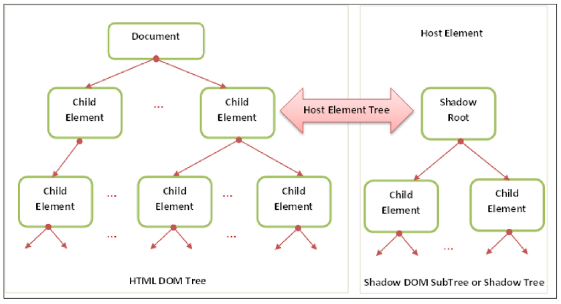
\includegraphics{shaDom.png}
				\caption{DOM und Shadow \ac{DOM} }
				\label{img:shaDom}
			\end{figure}
			Die Folge dieser Kapselung ist, dass alles was dem \emph{Shadow tree} hinzugefügt wird, nur lokal Einfluss auf diesen hat. Die Gestaltung von Webelementen im \emph{Shadow root} wird dadurch vereinfacht.
			\ac{CSS} Selektoren können somit nicht von außerhalb des \emph{Shadow roots} auf dieses Zugreifen und Selektoren, welche innerhalb dieses definiert werden haben keinen Einfluss auf den normalen \ac{DOM}.\smfootcite{Bidelman2016}
			
				
	\chapter{Methodik dieser Arbeit}
	\chapter{Adaptive Web Components}
		\section{Identifikation passender Web Components}
			\subsection{Identifikation Web Components}
			\subsection{Identifikation passender Preference Terms}
		\section{Preference Sets zur Adaptivität}
		\section{Adaptivität der bestehenden Web Components}
			\subsection{Web Component Eins}
				\subsubsection{Konzeption zur Adaptivität}
				\subsubsection{Umsetzung Programmierung}
			\subsection{Web Component Zwei}
			\subsection{Web Component Drei}
	\chapter{Vergleich}
		\section{Vergleich mit Polymer}

	\printbibliography

\end{document}